\documentclass{beamer}


\usepackage{color}
\usepackage{listings}
\usepackage{courier}
\lstset{
basicstyle=\tiny\ttfamily, % Standardschrift
numbers=left, % Ort der Zeilennummern
tabsize=4, % Groesse von Tabs
}
\lstloadlanguages{C++}
%\DeclareCaptionFont{blue}{\color{blue}}
 
%\captionsetup[lstlisting]{singlelinecheck=false, labelfont={blue}, textfont={blue}}
\usepackage{caption}
\DeclareCaptionFont{white}{\color{white}}
\DeclareCaptionFormat{listing}{\colorbox{8}{\parbox{\textwidth}{\hspace{15pt}#1#2#3}}}
\captionsetup[lstlisting]{format=listing,labelfont=white,textfont=white, singlelinecheck=false, margin=10pt, font={bf,footnotesize}}

\usepackage[utf8x]{inputenc}
\usepackage{ngerman}
\usepackage{graphicx}
\usepackage{amsmath}
\usepackage{amssymb}
\usepackage{amsthm}
\usepackage[arrow, matrix, curve]{xy}
\renewcommand{\phi}{\varphi}
\renewcommand{\epsilon}{\varepsilon}
\renewcommand{\bar}{\overline}
\newcommand{\R}{\mathbb{R}}
\newcommand{\C}{\mathbb{C}}
\newcommand{\N}{\mathbb{N}}
 \setbeamertemplate{theorems}[numbered]

\theoremstyle{definition} 
\newcounter{foo}
\newtheorem{df}[foo]{Definition}
\newtheorem{thm}[foo]{Theorem}
\newtheorem{kor}[foo]{Korrolar}
\newtheorem{ex}[foo]{Beispiel}
\newtheorem{lem}[foo]{Lemma}
\newtheorem{bem}[foo]{Bemerkung}
\newtheorem{prop}[foo]{Proposition}


\title{Dynamische Systeme}
\author{Matthias Hofmann}
\date{\today}

\usepackage{beamerthemesplit}


\begin{document}

\begin{frame}
	\titlepage
\end{frame}

\begin{frame}
	\frametitle{Inhaltsverzeichnis}
	\tableofcontents
\end{frame}

\section{Motivation: das Newton-Verfahren}
\begin{frame}
\frametitle{Motivation: das Newton-Verfahren}
Die Newtoniteration ist gegeben durch die Abbildung
\[
	\Phi(x)=z-\frac{f(z)}{f'(z)}
\]
Dabei ist für einen Startwert $z_0$ folgendes Verhalten denkbar
\begin{itemize}
\item Das Newton-Verfahren konvergiert gegen eine Nullstelle von $f$
\item Das Newton-Verfahren konvergiert nicht.
\end{itemize}

Das Newton-Verfahren konvergiert lokal. Wie ist das Konvergenzverhalten außerhalb dieser Konvergenzumgebung?

$\longrightarrow$ Newton-Fraktale.
\end{frame}

\begin{frame}
\begin{figure}
\centering
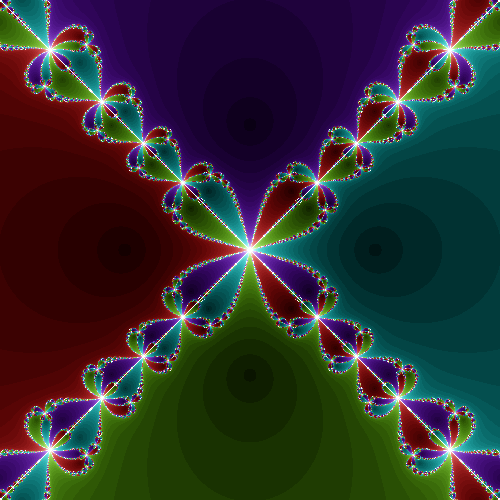
\includegraphics[scale=0.4]{fraktal.png}
\caption{Newton-Fraktal für $f(z)=z^4-1$}
\end{figure}
\end{frame}

\begin{frame}
Dies motiviert das Konzept der \emph{Fatou-} bzw. \emph{Juliamenge}:
\begin{description}
\item[Fatou-Menge] Die Startwerte aus dieser Menge führen unter Iteration zu einer ,,stetigen`` Dynamik, das heißt, eine kleine Änderung des Startwert führt zu einer ähnlichen Dynamik.
\item[Julia-Menge] Beschreibt die Menge der Startpunkte, die zu den ,,instabilen`` Prozessen gehören. Jede noch so kleine Änderung des Startwerts führt zu einer komplett anderen Dynamik.
\end{description} 
Notation: $F(f)$ bezeichnet die Fatoumenge von $f$ und $J(f)$ analog die Juliamenge von $f$.
\end{frame}

\begin{frame}
\frametitle{Charakterisierung periodischer Punkte}
\begin{df}
Sei $z_0$ periodischer Punkt bzgl. $f$ mit Periode n, d.h. $f^n(z_0)=z_0$. Dann heißt er
\begin{itemize}
\item \emph{stark anziehend}, falls $|(f^n)'(z_0)|=0$,
\item \emph{anziehend}, falls $0<|(f^n)'(z_0)|<1$,
\item \emph{indifferent}, wenn $|(f^n)'(z_0)|=1$,
\item \emph{abstoßend}, wenn $|(f^n)'(z_0)|>1$.
\end{itemize} 
\end{df}
\end{frame}

\begin{frame}
\begin{df}[Einzugsgebiet]
Ist $z_0$ ein anziehender periodischer Punkt von $f$, dann ist die Menge
\[
	A(z_0)=\{z\in \overline{\mathbb{C}}: \lim\limits_{L\ni k\to \infty} f^k(z)=z_0, L\subset \N\}
\]
das \emph{Einzugsgebiet} (engl. \emph{basin of attraction}) von $z_0$.
\end{df}
\end{frame}

\begin{frame}
\begin{df}[Julia-Menge]
Wir definieren die Julia-Menge durch
\[
J(f):=\overline{\{z\in \overline{\mathbb{C}}: z \text{ abstossender periodischer Punkt von $f$} \}}
\]
Und die Fatou-Menge durch $F(f)=J(f)^c$
\end{df}
\end{frame}

\section{Normale Familien und exzeptionelle Punkte}
\begin{frame}
\frametitle{Normale Familie und exzeptionelle Punkte}
\begin{df}
Eine Familie $\{F_n\}$ analytischer Funktionen operiert \emph{normal} auf $U$, falls jede Folge $(F_{n_i})_{i\in \mathbb{N}}$ eine Teilfolge $(F_{n_{i_j}})_{j\in \N}$ besitzt, sodass einer der beiden Eigenschaften erfüllt ist:
\begin{itemize}
\item $F_{n_{i_j}}$ konvergiert gleichmäßig auf kompakten Mengen $K\subset U$.
\item $F_{n_{i_j}}$ divergiert gleichmäßig gegen $\infty$ auf $U$.
\end{itemize}
Eine Familie $\{F_n\}$ analytischer Funktionen operiert \emph{nicht normal} bei $z_0$, falls er in keiner Umgebung \emph{normal} operiert.
\end{df}
\end{frame}

\begin{frame}
\begin{ex}
Betrachte die Funktion $F$, gegeben durch $F(x)=ax$. Definiere die Familie $\{F^n\}$.

\textbf{Fall 1: $|a|<1$.} so konvergiert für jede kompakte Teilmenge die Funktionenfolge $F^n(z)=a^n\cdot z$ gleichmäßig gegen 0. 

$\longrightarrow F(f)=\bar{\mathbb{C}}$, $A(0)=\C$, $A(\infty)=\{\infty\}$.

\textbf{Fall 2: $|a|>1$.} Die Familie $\{F\}$ operiert nicht normal bei $0$, denn für $z\neq 0$ divergiert jede beliebige Teilfolge.

$\longrightarrow J(F)=\{0\}$, $A(0)=\{0\}$, $A(\infty)=\bar{\C}\setminus \{0\}$. 
\end{ex}
\end{frame}

\begin{frame}
\begin{prop}
Sei $F$ analytisch, $z_0$ ein abstoßender periodischer Punkt. Dann operiert die Familie $\{F^n\}_{n\in \N}$ nicht normal bei $z_0$.
\end{prop}

\begin{kor}
Sei $F$ analytische Funktion. Die Familie $\{F^n\}$ operiert nicht normal für $z\in J(F)$.
\end{kor}
\end{frame}

\begin{frame}
\begin{thm}[Montels Theorem]
Sei $\{F_n\}$ eine Familie analytischer Funktionen auf einer Umgebung $U$. Angenommen es gibt $a,b \in \C, a\neq b$, sodass $F_n(z)\neq a \land F_n(z)\neq b$ für alle $n\in \N$ und $z\in U$. Dann operiert $\{F_n\}$ normal auf $U$. (ohne Beweis) 
\end{thm}

\begin{kor}
Sei $F$ eine analytische Funktion. Sei $z_0\in J(F)$ und sei $U$ eine beliebige Umgebung von $z_0$. Dann existiert höchstens ein $a\in \C$ mit
\[
	a\not\in \bigcup_{n=1}^\infty F^n(U).
\]
Wir nennen einen solchen Punkt \emph{exzeptionellen Punkt.}
\end{kor}
\end{frame}

\begin{frame}
\begin{thm}
Sei $P$ ein Polynom. Angenommen es gibt einen Punkt $z_0\in J(P)$ und ein $a\in \C$, sodass 
\[
\bigcup_{n=0}^\infty=\C\setminus\{a\}
\]
so folgt $P(z)=a+\lambda(z-a)^k$ für $\lambda \in \C, k\in \N$ geeignet. 
Insbesondere ist $P$ mit Grad $n\ge 2$ konjugiert zu $Q: z \mapsto z^n$, d.h. 
das ein Homöomorphismus $H$ existiert mit $Q\circ H=H\circ P$.
\end{thm}
\begin{bem}
Für $Q(z)=z^n, n\ge 2$ folgt $J(Q)=S^1$. Außerdem ist $a=0$ exzeptioneller Punkt.
\end{bem}
\end{frame}

\section{periodische Punkte}
\begin{frame}
\frametitle{periodische Punkte}
\begin{thm}[Koenigs Linearisationstheorem]
Sei $f$ eine analytische Funktion mit $f(0)=0$ und $f'(0)=\lambda$ mit 
$|\lambda|\neq0,1$, dann existiert ein lokaler Diffeomorphismus $\phi: U\to U$ mit 
$\phi(0)=0$, sodass 
\[
\phi \circ f(z)=\lambda\cdot \phi(z)
\] 
für $z\in U$. Dieses $\phi$ ist bis auf einen Multiplikation mit einer Konstanten eindeutig.
\end{thm}
\end{frame}

\begin{frame}
\begin{kor}
Sei $f:S \to S$ eine holomorphe Abbildung und $S$ eine Riemannsche Fläche mit anziehendem Fixpunkt $z_0$ mit $f'(z_0)=\lambda$. Sei $\Omega:=A(z_0)\cap S$ das Einzugsgebiet von $z_0$, dann gibt es eine holomorphe Abbildung $\phi$, so dass das Diagram

\begin{xy}
  \xymatrix{
      \Omega \ar[r]^f \ar[d]_\phi    &  \Omega \ar[d]^\phi  \\
      \C \ar[r]_{\lambda\cdot}             &   \C   
  }
\end{xy}

kommutiert, und $\phi$ eine Umgebung $U$ von  $z_0$ auf eine Umgebung von $0$ diffeomorph abbildet.
\end{kor}
\end{frame}

\begin{frame}
\begin{prop}
Sei $z_0$ ein anziehender periodischer Punkt, so existiert eine Umgebung $U$ um $z_0$, sodass $U\subset A(z_0)$. Wir nennen die Zusammenhangskomponente von $z_0\in A(z_0)$ auch das \emph{immediate Einzugsgebiet}.
\end{prop}

\begin{thm}
Sei P ein Polynom vom Grad $n\ge 2$ und sei $z_0$ ein anziehender periodischer Punkt von $P$. Dann liegt im Einzugsgebiet von $z_0$ ein kritischer Punkt.
\end{thm}
\end{frame}

\section{Eigenschaften der Julia-Menge}
\begin{frame}
\begin{prop}
\begin{itemize}
\item Sei P ein Polynom vom Grad $ n\ge 2$. Dann ist $J(P)\neq \emptyset$.
\item Für beliebige $n\in \N$ ist $J(P)=J(P^n)$.
\end{itemize}
\end{prop}

\begin{thm}
$J(P)=\{z|\{P^n\} \text{ operiert nicht normal auf } z\}$. 
\end{thm}
\begin{kor}
\begin{itemize}
\item $J(P)$ ist perfekt.
\item $J(P)$ ist komplett invariant
\item Die Menge der homoclinic Punkte sind dicht in $J(P)$
\end{itemize}
\end{kor}
\end{frame}

\begin{frame}
\begin{prop}
Sei $z_0 \in J(P)$. Es ist
\[
J(P)=\overline{\bigcup_{k=0}^\infty P^{-k}(z_0)}.
\]
\end{prop}
\begin{kor}
$J(P)$ ist nirgends dicht. 
\end{kor}

\begin{thm}
$P$ ist chaotisch auf $J(P)$
\end{thm}
\end{frame}


\end{document}
